\documentclass[a4paper]{IEEEtran}
\usepackage[slovene]{babel}
\usepackage[utf8]{inputenc}
\usepackage[T1]{fontenc}
\usepackage{amsfonts, amsthm,amsmath}
\usepackage{graphicx}
\usepackage{caption}
\usepackage{subcaption}
\title{Ravninske krivulje s pitagorejskim hodografom}
\author{Jan Fekonja, Anže Marinko \\ IŠRM2, FMF \\ Predmet: Geometrijsko podprto računalniško oblikovanje}
\date{december 2018}
\newtheorem{theorem}{Izrek}
\newtheorem{remark}{Opomba}
\newtheorem{lemma}{Lema}

\begin{document}
	\maketitle
	%\tableofcontents
	
	\section{Uvod}
	hodograf parametrične krivulje $r (t)$ v $\mathbb{R}^n$ je odvod krivulje same $r\prime (t)$ podan kot parametrična krivulja. Polinomska krivulja $r (t)$ v $\mathbb{R}^n$ je krivulja s Pitagorejskim hodografom (PH), če vsota kvadratov vseh $n$ polinomov na koordinatnih komponentah hodografa krivulje sovpada s kvadratom nekega polinoma $\sigma(t)$.
	Oglejmo si ravninske krivulje s PH.
	
	\section{Ravninske krivulje s Pitagorejskim hodografom}
	Ključna lastnost, ki razlikuje ravninsko krivuljo s PH $r (t) = (x (t), y (t))$ od "navadne" polinomske krivulje je privzeta vključitev Pitagorejskega pogoja v svoj hodograf, in sicer komponente $r\prime (t) = (x\prime (t), y\prime (t))$ morajo zadoščati pogoju $$x\prime^2(t) + y\prime^2(t)= \sigma^2 (t)$$ za nek polinom $\sigma(t)$. To lastnost je dosežena z upoštevanjem sledeče karakterizacije Pitagorejskih trojic polinomov.
	\begin{theorem}
		Pitagorejski pogoj
		\begin{equation} \label{eq:1}
		a^2 (t) + b^2 (t) = c^2 (t)
		\end{equation}
		izpolnjujejo polinomi $a (t), b (t), c (t)$ natanko tedaj, ko jih lahko izrazimo z drugimi polinomi $u (t), v (t), w (t)$ v obliki
		\begin{eqnarray} \label{eq:2}
		a (t) &=& \lbrack u^2(t)-v^2(t)\rbrack w(t),\nonumber\\
		b(t) &=& 2u(t)v(t)w(t),\\
		c(t) &=& \lbrack u^2(t)+v^2(t)\rbrack w(t),\nonumber
		\end{eqnarray}
		kjer imata $u(t)$ in $v(t)$ paroma različne ničle.
	\end{theorem}
	\proof
	Očitno je pogoj \eqref{eq:2} zadosten za \eqref{eq:1}. Potrebnost pogoja pa je dokazana v \cite{knjiga} na strani 382.
	\endproof
	\begin{remark} 
		Rešitve, kjer je $w(t)$ konstantna, imenujejo primitivne Pitagorejske trojice.
	\end{remark}
	Tedaj je ravninska krivulja s PH $r (t) = (x (t), y (t))$ definirana z zamenjavo treh polinomov $u (t), v (t), w (t)$ v izrazih
	\begin{eqnarray}\label{eq:3}
	x\prime(t) &=& \lbrack u^2(t)-v^2(t)\rbrack w(t)\\
	y\prime(t)&=&2u(t)v(t)w(t)\nonumber
	\end{eqnarray}
	in z integriranjem.
	
	Vsak nekonstantni skupni faktor $u (t)$ in $v (t)$ lahko absorbiramo v $w (t)$. Poleg tega moramo dopustiti določene izbire za $w (t), u (t), v (t)$, ki dajejo "degenerirane" krivulje s PH:
	\begin{enumerate}
		\item če je $w (t) = 0$ ali $u (t) = v (t) = 0$, je dobljeni hodograf $x\prime (t) = y\prime (t) = 0$ in definira eno točko namesto zveznega loka,
		\item če so $w (t), u (t), v (t)$ vse konstante (z $w$ in vsaj eno od $u$, $v$ neničelno) dobimo enakomerno parametrizirano premico, trivialno krivuljo s PH,
		\item če sta $u (t)$ in $v (t)$ konstanti, kjer je vsaj ena različna od nič in $w (t)$ ni konstanta, je dobljen lok spet linearen, vendar njegova parametrična hitrost ni konstantna (v splošnem),
		\item prav tako nastanejo nekonstantno parametrizirani linearni loki (vzporedni z osjo x), če je $w (t)\not = 0$ in je eden od $u (t)$ in $v (t)$ nič.
	\end{enumerate}
	V nadaljevanju bomo obravnavali le primere, kjer so $w (t), u (t), v (t)$ vse neničelne,
	in $u (t), v (t)$ nista obe konstanti.
	\begin{remark}
		Če je $w$ polinom stopnje $\lambda$ in je $\mu$ večja izmed stopenj polinomov $u$ in $v$, je krivulja s PH dobljena z integracijo hodografa (\ref{eq:3}) stopnje $n = \lambda + 2\mu+ 1$.
	\end{remark}

	\section{B\'ezierjeve kontrolne točke krivulj s PH}
	Osredotočimo se predvsem na primitivne Pitagorejske hodografe ($u$ in $v$ brez skupne ničle, $w(t)=1$). Taki hodografi definirajo regularne krivulje s PH, ki zadoščajo $r\prime (t)\not = 0$ za vse $t$. Točka na parametrični krivulji, kjer je $r\prime (t)=0$, je neregularna točka - običajno je to konica ali nenaden obrat tangente. Uporaba nekonstantnega polinoma $w (t)$ naredi konice (kar je nezaželena lastnost) na ustrezni krivulji s PH, če ima $w (t)$ realne ničle znotraj domene parametra krivulje. Krivulje s PH definirane z integracijo (\ref{eq:3}) primitivnih hodografov so lihe stopnje, $n = 2\mu + 1$.
	
	Najenostavnejše netrivialne krivulje s PH dobljene z $w (t) = 1$ in linearnima Bernsteinovima polinomoma:
	\begin{eqnarray}
	u (t) &=& u_0 B^1_0(t) + u_1 B^1_1(t),\nonumber\\
	v (t) &=& v_0 B^1_0(t) + v_1 B^1_1(t),\nonumber
	\end{eqnarray}
	ki zadoščajo $u_0v_1 - u_1v_0\not = 0$ in $(u_1 - u_0)^2+ (v_1 - v_0)^2\not = 0$, tako da imata $u (t), v (t)$ različne ničle in nista obe konstanti, nam dajo hodograf
	\begin{eqnarray}
	x\prime (t) &=& (u^2_0- v^2_0)B^2_0(t) +\nonumber\\
	& & (u_0u_1-v_0v_1)B^2_1(t)+(u^2_1-v^2_1)B^2_2(t),\nonumber\\
	y\prime(t) &=& 2u_0v_0B^2_0(t)+(u_0v_1+u_1v_0)B^2_1(t)+2u_1v_1B^2_2(t).\nonumber
	\end{eqnarray}
	Z integracijo tega hodografa dobimo kubično krivuljo s PH z B\'ezierjevimi kontrolnimi točkami oblike
	\begin{eqnarray}
	\textbf{p}_1 &=& \textbf{p}_0 + \frac{1}{3}(u_0^2-v_0^2,2u_0v_0),\nonumber\\
	\textbf{p}_2 &=& \textbf{p}_1 + \frac{1}{3}(u_0u_1-v_0v_1,u_0v_1+u_1v_0),\nonumber\\
	\textbf{p}_3 &=& \textbf{p}_2 + \frac{1}{3}(u_1^2-v_1^2,2u_1v_1),\nonumber
	\end{eqnarray}
	kjer je kontrolna točka $\textbf{p}_0$ definirana z integracijsko konstanto prosto izbrana.
	
	Krivulje pete stopnje s PH pa lahko definiramo s kvadratičnimi polinomi:
	\begin{eqnarray}
	u(t) &=& u_0B_0^2(t)+u_1B_1^2(t)+u_2B_2^2(t),\nonumber\\
	v(t)&=&v_0B_0^2(t)+v_1B_1^2(t)+v_2B_2^2(t),\nonumber
	\end{eqnarray}
	in z integracijo dobimo B\'ezierjeve kontrolne točke oblike:
	\begin{eqnarray}
	\textbf{p}_1 &=& \textbf{p}_0 + \frac{1}{5}(u_0^2-v_0^2,2u_0v_0),\nonumber\\
	\textbf{p}_2 &=& \textbf{p}_1 + \frac{1}{5}(u_0u_1-v_0v_1,u_0v_1+u_1v_0),\nonumber\\
	\textbf{p}_3 &=& \textbf{p}_2 + \frac{2}{15}(u_1^2-v_1^2,2u_1v_1)+\nonumber\\
	& & \frac{1}{15}(u_0u_2-v_0v_2,u_0v_2+u_2v_0),\nonumber\\
	\textbf{p}_4 &=& \textbf{p}_3 + \frac{1}{5}(u_1u_2-v_1v_2,u_1v_2+u_2v_1),\nonumber\\
	\textbf{p}_5 &=& \textbf{p}_4 + \frac{1}{5}(u_2^2-v_2^2,2u_2v_2),\nonumber
	\end{eqnarray}
	kjer je $\textbf{p}_0$ ponovno poljubna, velja pa
	$$(u_2v_0-u_0v_2)^2\not=4(u_0v_1-u_1v_0)(u_1v_2-u_2v_1).$$
	
	\begin{figure}[h]
		\centering
		\begin{subfigure}{.4\textwidth}
			\centering
			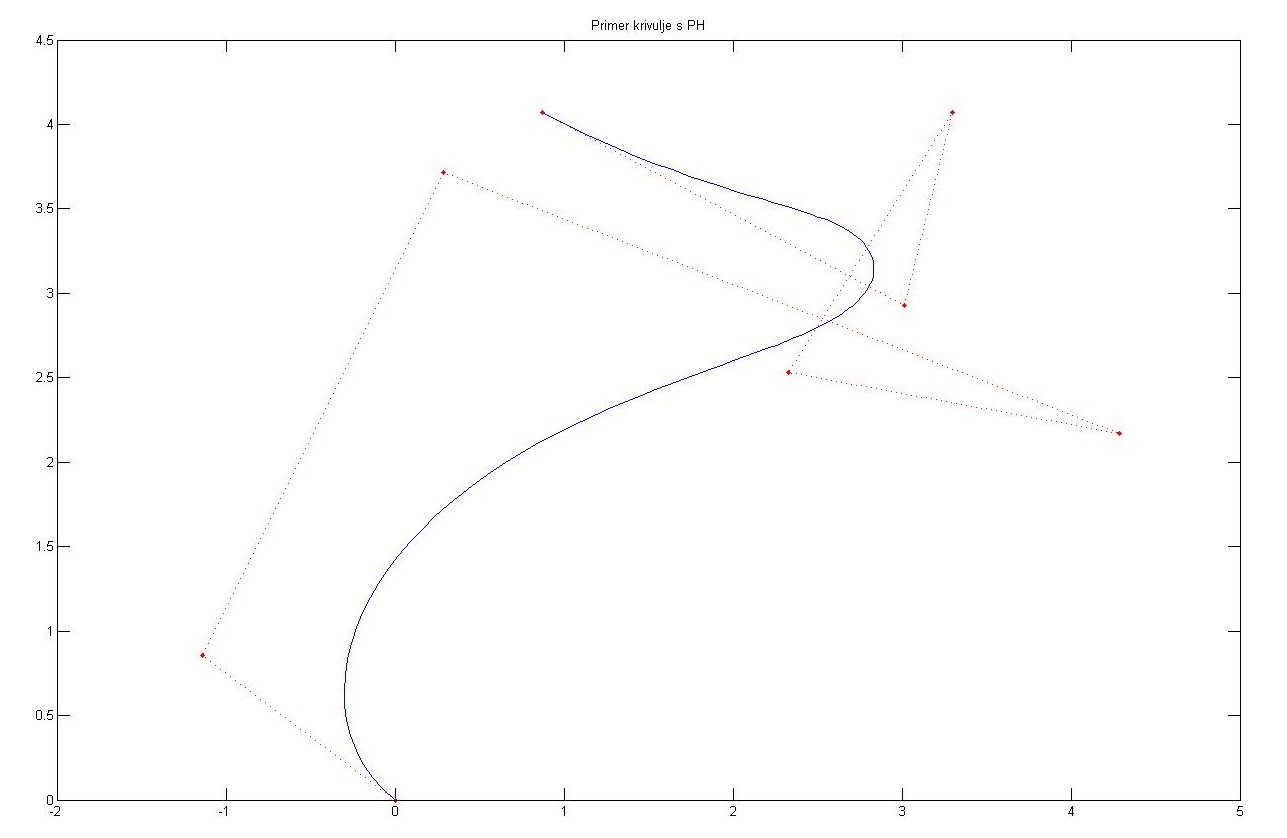
\includegraphics[width=\linewidth]{n3m2.jpg}
			\caption{Primer, kjer je stopnja $u$ 2, stopnja $v$ pa 3.}
			\label{fig:n2m3}
		\end{subfigure}%
	
		\begin{subfigure}{.4\textwidth}
			\centering
			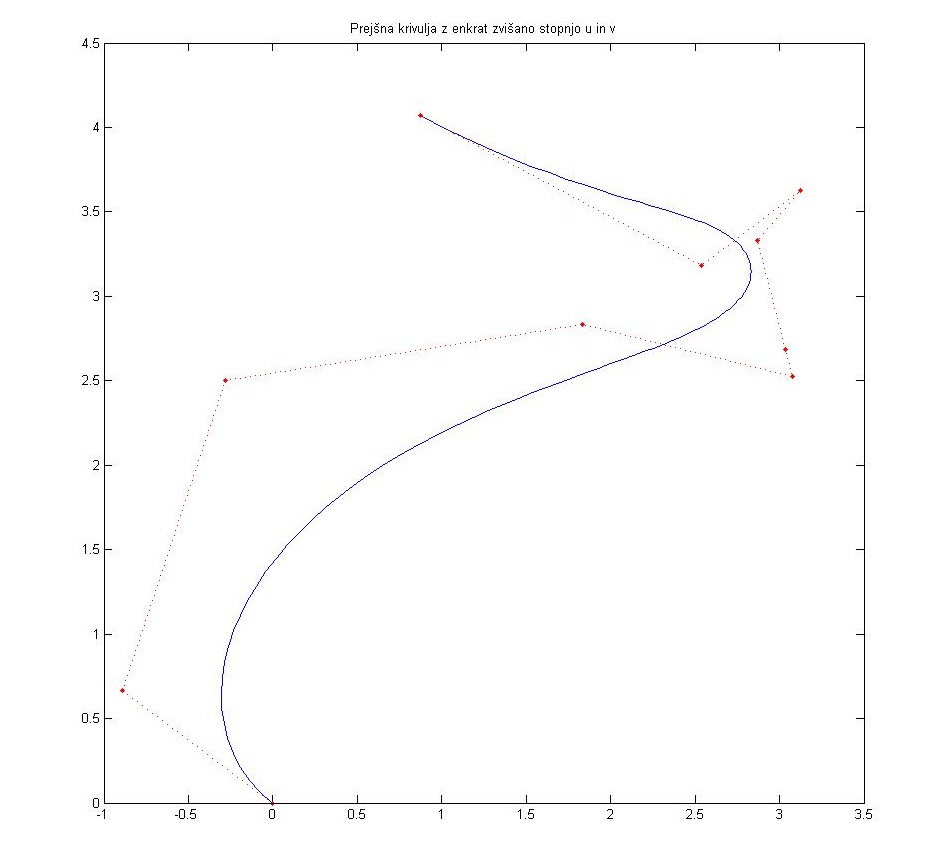
\includegraphics[width=\linewidth]{n4m3.jpg}
			\caption{Ista krivulja kot levo z enkrat zvišano stopnjo $u$ in $v$.}
			\label{fig:n3m4}
		\end{subfigure}
		\label{fig:nm}
	\end{figure}

	\section{Parametrična hitrost in dolžina loka}
	Parametrična hitrost regularne krivulje s PH $r (t) = (x (t), y (t))$ je podana s 
	$$\sigma (t) = | r\prime (t) | =\sqrt{x\prime^2(t)+y\prime^2(t)}= u^2 (t) + v^2 (t),$$
	in je polinom v $t$. Če je $r (t)$ (lihe) stopnje $n$, morata biti $u (t)$ in $v (t)$ stopinje $m = \frac{1}{2}(n - 1)$ in je lahko zapisan v Bernsteinovi obliki kot
	\begin{eqnarray}
	u (t) &=&\sum_{k=0}^m u_kB_k^m(t),\nonumber\\
	v (t)&=&\sum_{k=0}^m v_kB_k^m(t).\nonumber
	\end{eqnarray}
	Torej je
	$$\sigma (t) =\sum_{k=0}^{n-1} \sigma_kB_k^{n-1}(t),$$
	kjer so koeficienti 
	$$\sigma_k =\sum_{j=max(0,k-m)}^{min(m,k)}\frac{\binom{m}{j}\binom{m}{k-j}}{\binom{n-1}{k}}(u_ju_{k-j}+v_jv_{k-j}),$$ $$k = 0,\ldots , n - 1.$$
	Za kubične krivulje s PH je npr. $\sigma (t)$ kvadratna in ima Bernsteinove koeficiente
	\begin{eqnarray}
	\sigma_0 &=& u^2_0+ v^2_0, \nonumber\\
	\sigma_1 &=& u_0u_1 + v_0v_1, \nonumber\\
	\sigma_2 &=& u^2_1+ v^2_1.\nonumber
	\end{eqnarray}
	Za krivulje pete stopnje s PH pa je $\sigma(t)$ kvadratična z Bernsteinovimi koeficienti
	\begin{eqnarray}
	\sigma_0&=&u_0^2+v_0^2,\nonumber\\
	\sigma_1&=&u_0u_1+v_0v_1,\nonumber\\
	\sigma_2&=&\frac{2}{3}(u_1^2+v_1^2)+\frac{1}{3}(u_0u_2+v_0v_2),\nonumber\\
	\sigma_3&=&u_1u_2+v_1v_2,\nonumber\\
	\sigma_4&=&u_2^2+v_2^2.\nonumber
	\end{eqnarray}
	
	Da bi integrirali $\sigma (t)$ in tako dobili dolžino loka $s$ kot polinomsko funkcijo parametra,
	$$s (t) =\int^t_0\sigma(\tau) d\tau,$$
	uporabimo integracijsko pravilo za Bernsteinove bazne polinome. To nam da
	$$s (t) =\sum^n_{k=0}s_k\binom{n}{k}(1-t)^{n-k}t^k=\sum_{k=0}^n s_kB^n_k(t),$$
	kjer je $s_0=0$ in $s_k=\frac{1}{n}\sum^{k-1}_{j=0}\sigma_j, k=1,\ldots,n.$
	
	Torej je skupna dolžina loka $S$ preprosto
	$S = s (1) = \frac{\sigma_0+\sigma_1+\ldots+\sigma_{n-1}}{n}.$
	Za izračun dolžine loka izseka krivulje s PH za $t\in\lbrack a, b\rbrack$ pa vzamemo kar razliko $s (b) -s (a)$.
	
	Podobno je veliko preprosteje določiti vrednost parametra $t_*$, do katerega je dolžina loka (merjeno od $t = 0$) enaka dani vrednosti $s_*$ - t.j. rešiti enačbo $s (t_*) = s_*$ za $t_*$.
	
	Običajno se $r (t)$ prikaže z vrednotenjem vrednosti parametrov $t_0,\ldots , t_N$, ki ustreza enotnemu prirastku parametra $\Delta t = t_k- t_{k- 1}, k = 1,\ldots , N$. Vendar pa s tem dobimo neenakomerno razmaknjene (po dolžini loka) točke $r (t_k)$ na krivulji, saj parametrična hitrost $\sigma (t)$ v splošnem ni konstantna.
	
	Vseeno, če parametrična hitrost krivulje s PH ni konstantna, lahko s $s (t)$ enostavno popravimo to težavo. Naj bodo $t_0,\ldots, t_N$ vrednosti parametrov točk, ki so enakomerno razporejene z razmakom dolžine loka $\Delta s = S / N$, tako da
	$$s (t_k) = k\Delta s, k = 1,\ldots , N - 1,$$
	kjer $t_0 = 0$ in $t_N = 1$. Sedaj iz $\sigma (t) = ds / dt$ in $\sigma (t)$ pozitivno za vse $t$, ko polinoma $u$ in $v$ nimata nobene skupne ničle, sledi, da je $s (t)$ monotono naraščajoča s $t$ in s tem za vsak $k$ vrednost $s$ pri $t_k$ leži med $t_{k - 1}$ in 1. Kot začetni približek vzamemo
	$$t^{(0)}_k = t_{k-1}+\frac{\Delta s}{\sigma(t_{k-1})}$$
	in izbolšujmo rezultat z uporabo Newton-Raphsonove iteracije
	$$t^{(r)}_k = t^{(r-1)}_k-\frac{s(t^{(r-1)}_k)-k\Delta s}{\sigma(t^{(r-1)}_k)}, r = 1, 2,\ldots.$$
	Zadošča že kakšna iteracija, da dosežemo zadovoljivo natančnost.
	
	\begin{figure}[h]
		\centering
		\begin{subfigure}{.4\textwidth}
			\centering
			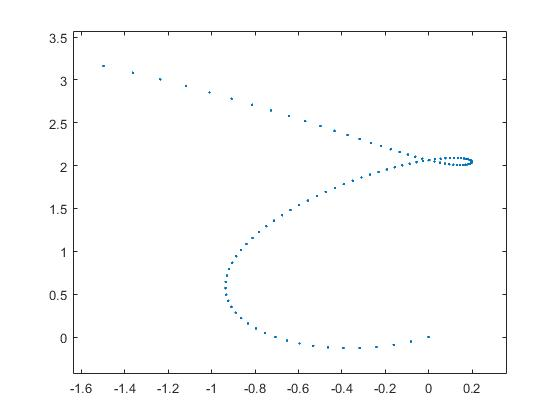
\includegraphics[width=\linewidth]{konstDt.jpg}
			\caption{$\Delta t=konst.$}
			\label{fig:constDt}
		\end{subfigure}%
	
		\begin{subfigure}{.4\textwidth}
			\centering
			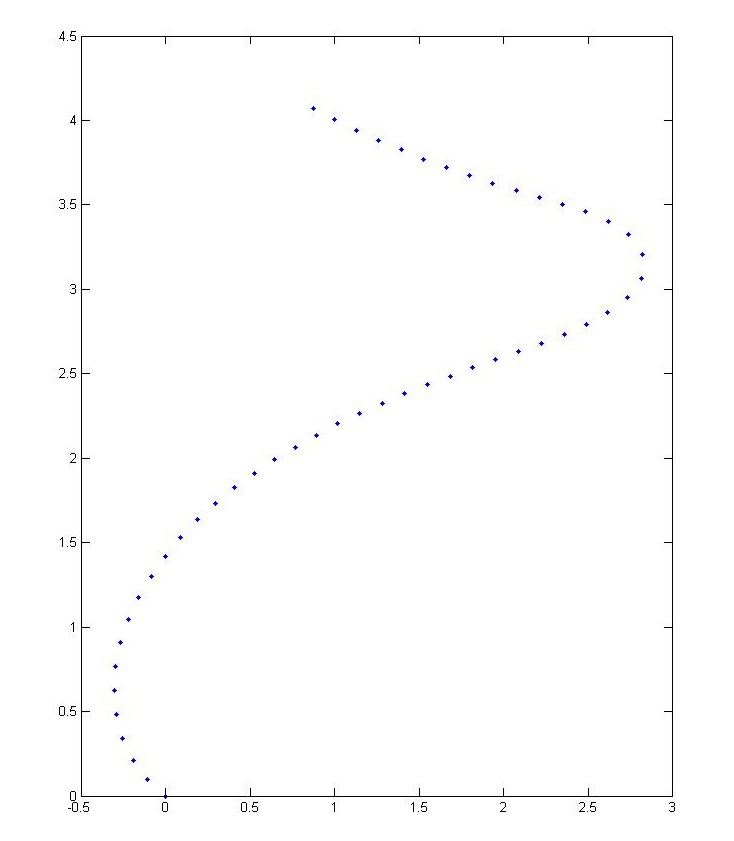
\includegraphics[width=\linewidth]{konstDs.jpg}
			\caption{$\Delta s=konst.$}
			\label{fig:constDs}
		\end{subfigure}
		\caption{Enakomerno povečanje parametra krivulje s PH (levo) in dolžine loka (desno) - parametrizacija po nekaj iteracijah. Prikaz točk na krivulji.}
		\label{fig:constD}
	\end{figure}
	
	\section{Lastnosti odvoda krivulje}
	Ker je parametrična hitrost krivulje s PH $r (t)$ definirane z integracijo polinom v $t$, imajo osnovne lastnosti njenih odvodov - enotski tangentni vektor, normala in ukrivljenost - racionalno odvisnost od parametra krivulje. Natančneje, definirani so v smislu polinomov $u (t)$ in $v (t)$, kjer
	$$\textbf{t} =\frac{(u^2 - v^2, 2uv)}{\sigma},\hspace{10pt} \textbf{n} =\frac{(2uv, v^2 - u^2)}{\sigma},\hspace{10pt} \kappa = 2 \frac{uv\prime - u\prime v}{\sigma^2}.$$
	
\begin{center}
	\begin{figure}[h]
		
		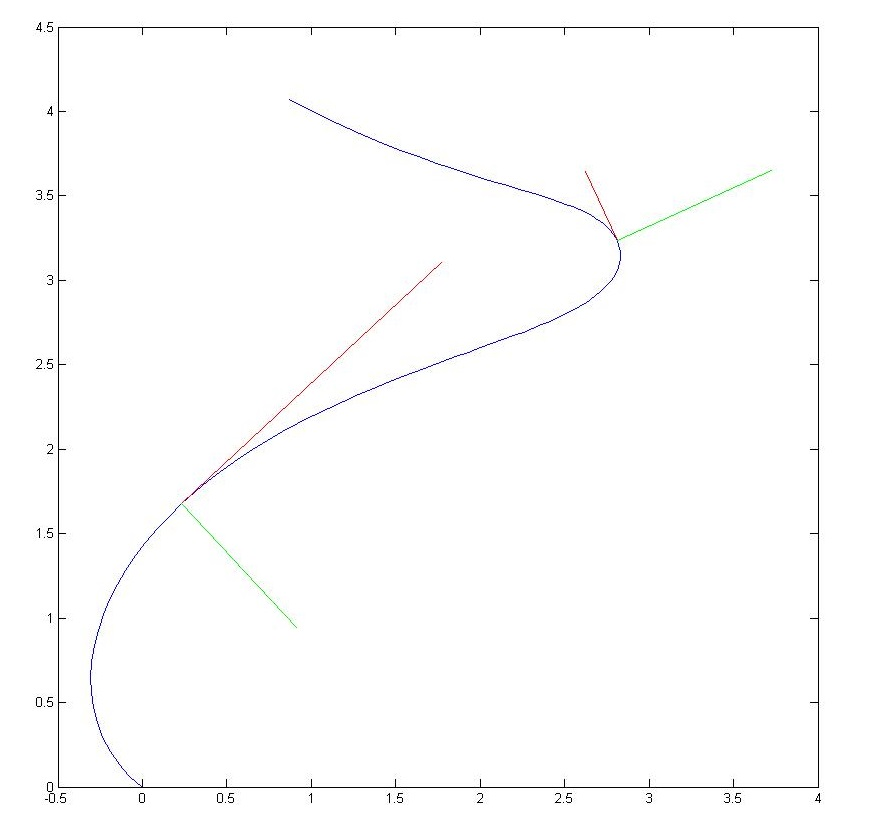
\includegraphics[width=0.7\linewidth]{tan-norm.jpg}
		\caption{$t = 0.2$ in $t = 0.7$}
		\label{fig:tan-norm}
	\end{figure}
\end{center}

	\section{Racionalni odmiki krivulj s PH}
	Odmiki pri vsaki razdalji $d$ od krivulje s PH $r (t)$, definirani kot
	$$r_d (t) = r (t) + d \textbf{n} (t),$$
	dovoljujejo natančno predstavitev v smislu racionalnih B\'ezierjevevih krivulj, ker je enotska normala $\textbf{n} (t)$ racionalno odvisna od parametra krivulje $t$. 
	
	Naj bodo kontrolne točke krivulje s PH $r (t)$ zapisane v homogenih koordinatah kot
	$$\textbf{P}_k = (W_k, X_k, Y_k) = (1, x_k, y_k),\hspace{20pt} k = 0,\ldots , n.$$
	Definirajmo prve diference kot
	$$\Delta\textbf{P}_k = \textbf{P}_{k + 1} - \textbf{P}_k = (0, \Delta x_k, \Delta y_k),\hspace{20pt} k = 0,\ldots, n - 1$$
	kjer je $\Delta x_k = x_{k + 1}- x_k, \Delta y_k = y_{k + 1}- y_k$. Naj bo $\Delta\textbf{P}_k^\perp = (0, \Delta y_k, -\Delta x_k).$
	
	Odmik za razdaljo $d$ od krivulje s PH $r (t)$ je definiran zgoraj z $r_d(t)$, kjer je normala $\textbf{n}(t)$ na $r (t)$ podana zgoraj. Odmik lahko izrazimo kot
	$$r_d (t) = \left(\frac{X (t)}{W(t)},\frac{Y(t)}{W(t)}\right),$$
	kjer so $W (t), X (t), Y (t)$ polinomi stopnje $2n - 1$, katerih koeficienti
	$$\textbf{O}_k = (W_k, X_k, Y_k), \hspace{10px} k = 0,\ldots , 2n - 1,$$
	določajo B\'ezierjeve kontrolne točke racionalne krivulje odmika.
	
	Homogene koordinate za kontrolne točke odmika so lahko strnjeno izražene v smislu prvotne krivulje kot
	$$\textbf{O}_k =\sum^{min (n - 1, k)}_{j = max (0, k - n)}\frac{\binom{n-1}{j}\binom{n}{k-j}}{\binom{2n-1}{k}}(\sigma_j\textbf{P}_{k-j}+dn\Delta\textbf{P}_j^\perp),$$ $$k = 0,\ldots, 2n - 1.$$
	
	S tem dobimo za kubične krivulje s PH 6 kontrolnih točk racionalnih odmikov kot krivulj pete stopnje, za krivulje s PH pete stopnje pa dobimo 10 kontrolnih točk racionalnih odmikov kot krivulj devete stopnje.
	
\begin{center}
\begin{figure}[h]
	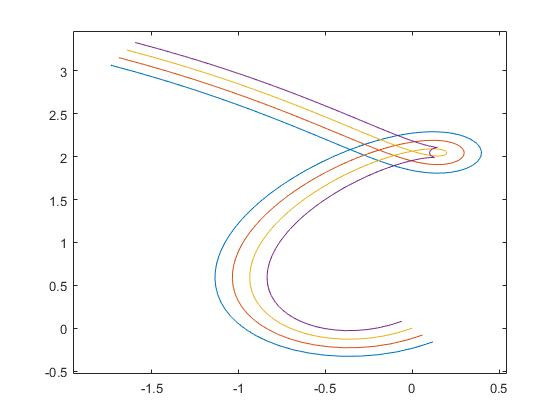
\includegraphics[width=0.7\linewidth]{odmik.jpg} 
	\caption{Krivulja s PH (rdeča) in racionalni odmiki za $d=-0.6,-0.5,\ldots,0.5,0.6$.}
	\label{fig:odmik}	
\end{figure}
\end{center}
	
	Opazimo, da so racionalni odmiki eksaktni za vsak $d$ tudi v primeru špic in ko krivulja prečka samo sebe.
	
	
	% Jan
	\section{Kompleksna predstavitev}
	Kompleksna predstavitev $\mathbb{R}^2$ je še posebej dragocena v analizi ravninskih krivulj s PH, saj ponuja enostavno in eleganto karekterizacijo lastnosti pitagorejskih hodografov. Vse kaj lahko naredimo s kompleksno predstavitvijo bi načeloma lahko dosegli z uporabo samo realnih spremenljivk. Vendar zaradi uporabnih geometrijskih vpogledov, ki jih nudi, se močno zanašamo na kompleksno predstavitev ravninskih krivulj s PH.
	
	\section{Kompleksne krivulje in hodografi}
	Vpeljemo presikavo hodografske ravnine, to je ravnina, v kateri je odvod $r\prime (t)$ parametrične krivulje $r(t)$. S to shemo uvedemo korespondenco ena na ena med množicamo regularnih krivulj s PH in regularnih "navadnih" polinomskih krivulj, ki nudi ogrudje za primerjavo in razlikovanje njunih lastnosti.
	
	Imejmo polinomsko krivuljo v kompleksni ravnini, ki je v B\'ezierjevi obliki
	
	\begin{equation} \label{eq:4}
	r(t) = \displaystyle\sum_{k=0}^{n} p_k \binom{n}{k} (1-t)^{n-k}t^k, \ t \in [0,1],
	\end{equation}
	kjer kompleksne vrednosti $p_k=x_k+iy_k$, $k=0,...,n$ določajo kontrolne točke. Hodograf $w(t)=r\prime (t)$ krivulje \ref{eq:4} izrazimo kot kompleksno B\'ezierjevo krivuljo stopnje $n-1$,
	
	\begin{equation} \label{eq:5}
	w(t)=\displaystyle\sum_{k=0}^{n-1} w_k \binom{n-1}{k}(1-t)^{n-1-k}t^k, \ t \in [0,1],
	\end{equation}
	s kontrolnimi točkami
	\begin{equation}
	w_k=n \Delta p_k = n(p_{k+1}-p_k), \ k=0,...,n-1.
	\end{equation}
	
	Razlike $\Delta p_k = p_{k+1}-p_k$ določajo $n$ usmerjenih "nog" kontrolnega poligona. Zaradi jasnosti obravnavamo krivulje in njene hodografe v dveh ločenih kompleksnih ravninah $z=x+iy$ in $w=u+iv$.
	
	\section{Korespondenca ena na ena}
	Uporabimo $\mathbb{C}$ za predstavitev $\mathbb{R}^2$. Naj bo $\Pi$ množica vseh regularnih polinomskih krivulj in naj bo $\hat{\Pi}$ množica vseh regularnih krivulj s PH. Čeprav sta $\pi$ in $\hat{\Pi}$ neskončni množici, saj obe vsebujeta krivulje poljubnih stopenj, je jasno, da velja $\hat{\Pi} \subset \Pi$, saj vsaka regularna krivulje s PH je tudi regularna polinomska krivulja, vendar obstajajo regularne polinomske krivulje, katerih hodografi niso Pitagorejski (na primer, parabola $r(t) = t + i t^2$). 
	
	Preprost tristopenski postopek $P$, ki pretvori poljubno odvedljivo ravninsko krivuljo $r(t)$ v novo krivuljo $\hat{r}(t)$:
	\begin{enumerate}
	\item odvedemo dano krivuljo $r(t)$, da dobimo njen hodograf $w(t)=r'(t)$;
	\item uporabimo preslikavo $w \rightarrow w^2$ mad ravninskim hodografom, da dobimo $\hat{w}(t)=w^2(t)$;
	\item integriramo preslikan hodograf $\hat{w}(t)$, da dobimo novo krivuljo $\hat{r}(t)= \int \hat{w}(t)dt$.
	\end{enumerate}
	V tem postopku predpostavimo $r(0)= \hat{r}(0) = 0$.
	
	\begin{theorem}
	$P$ definira bijektivno preslikavo ali krespodenco ena na ena med množicamoa $\Pi$ in $\hat{\Pi}$ ragularnih polinomskih krivulj in regularnih PH krivulj.
	\end{theorem}
	
	\proof
	Dokaz v \cite{knjiga} na straneh 409 in 410.
	\endproof
	
	V splošnem velja, da z inverzno preslikavo $w \rightarrow \sqrt{w}$ ne  dobimo polinomskega hodografa, kadar jo uporabimo na splošnem polinomskem hodografu. Pravzaprav dobimo polinomski hodograph samo kadar jo uporabimo na Pitagorejskem hodografu. Torej velja $P(\Pi) = \hat{\Pi}$ in $P^{-1}(\hat{\Pi}) = \Pi$.
	
	Če sta regularna polinomska krivulja $r(t)$ in regularna krivulja s PH $\hat{r}(t)$ med sebom povezani s preslikavama $P$ in $P^{-1}$m potem lahko takšne pare izrazimo kot:
	
	\begin{eqnarray}\label{eq:6}
	r(t) = \int_0^t u( \tau ) d \tau + i \int_0^t v( \tau ) d \tau , \nonumber \\
	\hat{r}(t) = \int_0^t (u^2( \tau ) - v^2( \tau ) d \tau ) + i \int_0^t 2 u( \tau ) v( \tau ) d \tau ,
	\end{eqnarray}	
	
	kjer sta $u(t)$ in $v(t)$ razmeroma preprosta polinoma in predpostavimo $r(0) = \hat{r}(0) = 0$.
	
	\begin{remark}
	Množica $\hat{\Pi}$ regularnih krivulj s PH ima enako kardinalnost ali moč kot množica $\Pi$ regularnih polinomskih krivulj.
	\end{remark}
	
	\begin{lemma}
	Stonji $n$ in $\hat{n}$ pripadajočima krivuljama $r(t)$ in $\hat{r}(t)$ sta povezani z $\hat{n}=2n-1$.
	\end{lemma}
	
	\proof
	Pri postopku $P$ najprej odvajamo krivuljo $r(t)$ stopnje $n$ in dobimo njen hodograf $w(t)$ stopnje $n-1$. Nato kvadriramo $w(t)$  in dobimo hodograf $\hat{w}(t)$ stopnje $2n-2$. Na koncu integriramo $\hat{w}(t)$ in dobimo novo krivuljo $\hat{r}(t)$ stopnje $2n-1$.
	\endproof
	
	Očitno ne obstajajo  regularne krivulje s PH, ki so sode stopnje. Ravne črte v $\Pi$ ustrezajo (drugačnim) ravnim črtam v $\hat{\Pi}$, ampak $P$ preslika regularne polinomske krivulje stopnje $\geq 2$ v regularne krivulje s PH višje lihe stopnje (glej tabelo \ref{table:1}).
	
	\begin{center}
	\begin{table}
	\caption{Ujemajoče se krivulje nižjih stopenj.}
	\label{table:1}
	\begin{tabular}{c c c}
	\hline
	& polinomska krivulja $r(t)$ & krivulja s PH $\hat{r}(t)$ \\
	\hline
	$n=1$ & ravne črte & ravne črte \\
	$n=2$ & parabole & Tschirnhausove kubične krivulje \\
	$n=3$ & regularne kubične krivulje & regularni kvintiki s PH \\
	\vdots & \vdots & \vdots \\
	\hline
	\end{tabular}
	\end{table}
	\end{center}
	
	\begin{theorem}
	Kontrolne točke regularne krivulje s PH stopnje $2n-1$ so podane kot $n$ kompleksnih vrednosti $w_0 ,..., w_{n-1}$ z rekurzivno formulo
	\begin{equation} \label{eq:7}
	p_{k+1} = p_k + \frac{1}{2n-1} \displaystyle\sum_{j=max(0,k-n+1}^{min(k,n-1} \frac{\binom{n-1}{j} \binom{n-1}{k-j}}{\binom{2n-2}{k}} w_j w_{k-j}
	\end{equation}
	za $k=0,1,...,2n-2$, kjer je $p_0$ poljuben in $w_0,...,w_{n-1}$ so takšni, da hodograf $w(t)$ definiran v (\ref{eq:4}) ne pokvari originalnega.
	\end{theorem}
	
	\proof
	Dokaz v \cite{knjiga} na strani 413.
	\endproof
	
	
	\section{Rotacijske invariance hodografov}
	Kompleksna predstavite ponuja preprost dokaz za rotacijsko invariantnost zadostne in potrebne oblike
	
	\begin{eqnarray}
	x \prime (t)=u^2(t)-v^2(t), \nonumber \\
	y \prime (t)=2u(t)v(t), \\
	\sigma (t)=u^2(t)+v^2(t)\nonumber 
	\end{eqnarray}
	
	za primitivne ravninske pitagorejske hodografe $r\prime (t)=(x\prime (t),y\prime (t))$ zadošča
	
	\begin{equation}
	x \prime ^2 (t) + y \prime ^2 (t) = \sigma ^2 (t),
	\end{equation}

	kjer $D(u,v)=konstanta \Rightarrow gcd(x\prime ,y\prime )=konstanta$. Ob rotaciji
	
	\begin{equation}
	\begin{bmatrix}
	\widetilde{x} \prime (t) \\
	\widetilde{y} \prime (t)
	\end{bmatrix}
	=
	\begin{bmatrix}
	cos \theta & -sin\theta \\
	sin\theta & cos\theta
	\end{bmatrix}
	\begin{bmatrix}
	x \prime (t) \\
	y \prime (t)
	\end{bmatrix}
	\end{equation}
	po kotu $\theta$, poskužamo izraziti rotacijski hodograf $\widetilde{r} \prime (t) = (\widetilde{x} \prime (t),\widetilde{y} \prime (t))$ v smislu dveh novih polinomov $\widetilde{u} (t)$, $\widetilde{x} (v)$ kot
	
	\begin{equation} \label{eq:8}
	\widetilde{x} \prime (t) = \widetilde{u}^2 (t) - \widetilde{v}^2 (t), \ \widetilde{y} \prime (t) = 2 \widetilde{u} (t) \widetilde{v} (t).
	\end{equation}
	
	Opazimo lahko, da je preoblikovan hodograf,
	\begin{eqnarray}
	\widetilde{x} \prime (t) = cos \theta [\widetilde{u}^2 (t) - \widetilde{v}^2 (t)] - sin\theta 2u(t)v(t), \nonumber \\
	\widetilde{y} \prime (t) = sin \theta [\widetilde{u}^2 (t) - \widetilde{v}^2 (t)] + cos\theta 2u(t)v(t),
	\end{eqnarray}

	dobljen z vstavljanjem polinomov v (\ref{eq:8})
	
	\begin{eqnarray}\label{eq:9}
	\widetilde{u} (t)=cos\frac{1}{2}\theta u(t)-sin\frac{1}{2}\theta v(t), \nonumber \\
	\widetilde{v} (t)=sin\frac{1}{2}\theta u(t)+cos\frac{1}{2}\theta v(t). 
	\end{eqnarray}
	
	Z uporabo kompleksne predstavitve $r\prime (t)=w^2(t)$, kjer je $w(t)=u(t)+iv(t)$, pri rotaciji dobimo $\widetilde{r}\prime (t)=exp(i\theta )w^2(t)=\widetilde{r}\prime (t)=\widetilde{w}^2 (t)$, kjer je realni in imaginarni del $\widetilde{w}=exp(i\frac{1}{2}\theta )w(t)=\widetilde{u} (t)+ i\widetilde{v} (t)$ definiran z (\ref{eq:9}).
	
	
	\section{Karekterizacija krivulje pete stopnje s PH}
	Kontrolne točke (\ref{eq:7}) za krivulje pete stopnje s PH so oblike
	
	\begin{eqnarray}\label{eq:10}
	p_1=p_0+\frac{1}{5}w_0^2, \nonumber \\
	p_2=p_1+\frac{1}{5}w_0w_1, \nonumber \\
	p_3=p_2+\frac{1}{5}\frac{2w_1^2+w_0w_2}{3}, \nonumber \\
	p_4=p_3+\frac{1}{5}w_1w_2, \nonumber \\
	p_5=p_4+\frac{1}{5}w_2^2. 
	\end{eqnarray}
	
	Z uporabo kompleksne oblike dobimo karakterizacijo za krivulje pete stopnje s PH v smislu geometrije kontrolnih poligonov. Ponovno zapišemo enačbe (\ref{eq:10}) v smislu $\Delta p_k=p_{k-1}-p_k$ kot
	
	\begin{eqnarray}\label{eq:11}
	\Delta p_0=\frac{w_0^2}{5}, \ \Delta p_1=\frac{w_0w_1}{5}, \nonumber \\
	\Delta p_2=\frac{2w_1^2+w_0w_2}{15}, \nonumber \\
	\Delta p_3=\frac{w_1w_2}{5}, \ \Delta p_4=\frac{w_2^2}{5}.
	\end{eqnarray}
	Za regularne krivulje velja $\Delta p_0 \neq 0$ in $\Delta p_4 \neq 0$.
	
	\begin{theorem}
	Naj bodo noge kontrolnega polinoma regularne krivulje pete stopnje definirane kot kompleksne vrednosti $\Delta p_0,...,\Delta p_4$. Potem ima krivulja pitagorejski hodograf natanko tedaj, ko te vrednosti zadoščajo enačbi:
	\begin{equation}\label{eq:12}
	\Delta p_0(\Delta p_3)^2=\Delta p_4(\Delta p_1)^2,
	\end{equation}
	in se ujemajo z nasednjim sistemom umejitev:
	\begin{eqnarray}\label{eq:13}
	3\Delta p_0\Delta p_1\Delta p_2-(\Delta p_0)^2\Delta p_3-2(\Delta p_1)^3=0, \nonumber \\
	3\Delta p_4\Delta p_3\Delta p_2-(\Delta p_4)^2\Delta p_1-2(\Delta p_3)^3=0, \nonumber \\
	3\Delta p_0\Delta p_3\Delta p_2-\Delta p_4\Delta p_0\Delta p_1-2(\Delta p_1)^2\Delta p_3=0, \nonumber \\
	3\Delta p_4\Delta p_1\Delta p_2-\Delta p_0\Delta p_4\Delta p_3-2(\Delta p_3)^2\Delta p_1=0, \nonumber \\
	9\Delta p_0(\Delta p_2)^2-6(\Delta p_1)^2\Delta p_2-2\Delta p_0\Delta p_1 \Delta p_3-(\Delta p_0)^2\Delta p_4=0, \nonumber \\
	9\Delta p_4(\Delta p_2)^2-6(\Delta p_3)^2\Delta p_2-2\Delta p_4\Delta p_3 \Delta p_1-(\Delta p_4)^2\Delta p_3=0.
	\end{eqnarray}
	\end{theorem}
	
	Če sta oba $\Delta p_1$ in $\Delta p_3$ neničelna, potem enačba (\ref{eq:12}) in ena od prvih štirih enačb (\ref{eq:13}) predstavlja zadosten in potreben pogoj, da je krivulja pete stopnje krivulja s PH. Če $\Delta p_1=\Delta p_3=0$, potem (\ref{eq:12}) in prve štiri enačbe iz (\ref{eq:13}) postanejo identitete in moramo vzeti eno izmed dveh zadnjih enačb iz (\ref{eq:13}) za pogoj.
	
	\proof
	Dokaz v \cite{knjiga} na straneh 417 in 418.
	\endproof
	
	\section{Geometrija kontrolnega poligona}
	\iffalse
	Z izražanje nog kontrolnega poligona v polarni obliki $\Delta p_k=L_ke^{i\xi _k}, k=0,...,4$ dobimo $L_0L_1^2$ in $\xi _0+2\xi _3=\xi _4 + 2\xi _1$. Če prepišemo v smislu štirih notranjih kotov $\theta _i=\pi +\xi _i -\xi _{i-1}$ za $i=1,...,4$ vidimo, da je geometrija kontrolnega polinoma omejena z razmerji
	\begin{equation}\label{eq:14}
	\frac{L_1}{L_3}=\sqrt{\frac{L_0}{L_4}} \ in \ \theta _1+\theta _4 = \theta _2 + \theta _3.
	\end{equation}
	\fi
	
	\subsection{Samo štiti različne kontrolne točke}
	Ta primer nastopi, ko vzamemo $w_1=0$ v (\ref{eq:10}), torej je $p_1=p_2$ in $p_3=p_4$. Potem je kontrolni poligon naslednje oblike:
	\begin{eqnarray}
	\Delta p_0=\frac{w_0^2}{5}, \ \Delta p_1=0, \nonumber \\
	\Delta p_2 =\pm \frac{w_0w_2}{15}, \ \Delta p_3=0, \ \Delta p_4=\frac{w_2^2}{5}. \nonumber 
	\end{eqnarray}
	Čeprev imamo samo štiri različne kontrolne točke, ta hodogaf definira pravo krivuljo pete stopnje s PH, in ne kubično krivuljo s PH zvišane stopnje. Še več, ta krivulja je regularna, če velja $w_0,w_2 \neq 0$.
	
	\subsection{Samo pet različnih kontrolnih točk}
	V tem primeri je vrednost od $w_1$ izbrana tako, da velja $2w_1^2+w_0w_2=0$, in zato velja $p_2=p_3$. Tako velja, da je $\Delta p_2=0$ in ostale noge kontrolnega pogolina lahko izrazimo s samo $w_0$ in $w_2$:
	\begin{eqnarray}
	\Delta p_0=\frac{w_0^2}{5}, \ \Delta p_1=\pm i \frac{w_0}{5}\sqrt{\frac{w_0w_2}{2}}, \nonumber \\
	\Delta p_3 =\pm i\frac{w_2}{5}\sqrt{\frac{w_0w_2}{2}}, \ \Delta p_4=\frac{w_2^2}{5}. \nonumber
	\end{eqnarray}
	
	Za tako degenerirano obliko, sta pogoja (\ref{eq:12}) in (\ref{eq:13}) lahko reducirana na:
	
	\begin{eqnarray}
	\Delta p_0(\Delta p_3)^2 =\Delta p_4(\Delta p_1)^2,\nonumber \\
	\Delta p_0 \Delta p_4 + 2\Delta p_1 \Delta p_3 = 0.\nonumber
	\end{eqnarray}
	
	\subsection{Krivulja s PH povišane stopnje}
	Stopnjo katerekoli krivulje s PH je mogoče dvigniti, ne da bi pri tem ogrozili pitagorejsko naravo njenega hodografa, saj višanje stopnje pomeni le redundantno predstavitev. Če postopek višanje stopnje nanesemo dvakrat na kontrolni poligon kubične krivulje s PH, potem ima krivulja pete stopnje s PH kontrolne točke:
	
	\begin{eqnarray}\label{eq:15}
	p_1 = p_0 +\frac{1}{5}w_0^2, \nonumber \\
	p_2 = p_1 +\frac{1}{1}(w_0^2+w_0w_1), \nonumber \\
	p_3 = p_2 +\frac{1}{30}(w_0^2+4w_0w_1+w_1^2), \nonumber \\
	p_4 = p_3 +\frac{1}{10}(w_0w_1+w_1^2), \nonumber \\
	p_5 = p_4 +\frac{1}{5}w_1^2.
	\end{eqnarray}
	
	Preverimo lahko, da so enačbe (\ref{eq:15}) oblike (\ref{eq:10}) le da so $w_0,w_1,w_2$ zamenjani z $w_0,\frac{1}{2}(w_0+w_1), w_1$. Od tod sledi, da je vrednost $w_1$ v enačba (\ref{eq:10}) vedno povprečje vrednosti $w_0$ in $w_2$. 
	
	\begin{thebibliography}{1}
		\bibitem{knjiga} R. T. Farouki: Pythagorean-Hodograph Curves: Algebra and Geometry Inseparable, poglavje 17 in 19.
	\end{thebibliography}
\end{document}